% !TeX root = ../main.tex

\chapter{数据模拟细节}
\label{cpm:MC}

\begin{table}[ht]
      \centering
      \caption{隐藏区域模型模拟数据总结}
      \label{tab:signal_MC}
      \begin{tabular}{cccc}
            \toprule
            $m_\Phi$ [\GeV] & $m_s$ [\GeV]         & $c\tau$ [m] & 总事例数 (mc16a, mc16d, mc16e) \\
            \midrule
            \multirow{2}{*}{60}
                            & 5                    & 0.217       & 600k (160k, 190k, 250k)        \\
                            & 15                   & 0.661       & 300k (80k, 100k, 120k)         \\
            \midrule
            \multirow{7}{*}{125}
                            & \multirow{2}{*}{5}   & 0.127       & 160k (40k, 50k, 70k)           \\
                            &                      & 0.411       & 601k (160k, 190k, 251k)        \\
                            & 15                   & 0.58        & 510k (140k, 160k, 210k)        \\
                            & \multirow{2}{*}{35}  & 1.31        & 720k (190k, 230k, 300k)        \\
                            &                      & 2.63        & 509k (140k, 160k, 210k)        \\
                            & \multirow{2}{*}{55}  & 1.05        & 1010k (270k, 320k, 420k)       \\
                            &                      & 5.32        & 458k (120k, 150k, 188k)        \\
            \midrule
            200             & 50                   & 1.255       & 200k (50k, 70k, 80k)           \\
            \midrule
            400             & 100                  & 1.608       & 200k (50k, 70k, 80k)           \\
            \midrule
            \multirow{4}{*}{600}
                            & 50                   & 0.59        & 300k (80k, 100k, 120k)         \\
                            & \multirow{2}{*}{150} & 1.84        & 300k (80k, 100k, 120k)         \\
                            &                      & 3.309       & 150k (40k, 50k, 60k)           \\
                            & 275                  & 4.288       & 1000k (260k, 320k, 420k)       \\
            \midrule
            \multirow{4}{*}{1000}
                            & 50                   & 0.406       & 300k (80k, 100k, 120k)         \\
                            & \multirow{2}{*}{275} & 2.399       & 300k (80k, 100k, 120k)         \\
                            &                      & 4.328       & 150k (40k, 50k, 60k)           \\
                            & 475                  & 6.039       & 1000k (260k, 320k, 420k)       \\
            \bottomrule
      \end{tabular}
\end{table}

\begin{table}[ht]
      \centering
      \caption{标准模型多喷注背景模拟数据总结}
      \label{tab:background_MC}
      \begin{tabular}{*4{c}}
            \toprule
            样本编号 & 名称  & $p_{\mathrm{T}}$ 范围 [\GeV] & 产生 截面 $\sigma$ [pb] \\
            \midrule
            361022   & JZ2W  & 60 -- 160                    & $2.43 \times 10^{9}$    \\
            361023   & JZ3W  & 160 -- 400                   & $2.65 \times 10^{7}$    \\
            361024   & JZ4W  & 400 -- 800                   & $2.55 \times 10^{5}$    \\
            361025   & JZ5W  & 800 -- 1300                  & $4.55 \times 10^{3}$    \\
            361026   & JZ6W  & 1300 -- 1800                 & \num{2.58e2}            \\
            361027   & JZ7W  & 1800 -- 2500                 & \num{1.62e1}            \\
            361028   & JZ8W  & 2500 -- 3200                 & \num{6.25e-1}           \\
            361029   & JZ9W  & 3200 -- 3900                 & \num{1.96e-2}           \\
            361030   & JZ10W & 3900 -- 4600                 & \num{1.20e-3}           \\
            361031   & JZ11W & 4600 -- 5300                 & $4.23 \times 10^{-5}$   \\
            361032   & JZ12W & 5300 -- $\infty$             & $1.04 \times 10^{-6}$   \\
            \bottomrule
      \end{tabular}
\end{table}


\chapter{BDT 的输入变量}
\label{cpm:BDT}

以下是用于逐事件 BDT 训练的输入变量列表:

\begin{enumerate}
      \item 每个 CalRatio 候选信号喷注($\text{jet}^{\text{sig}1}$、$\text{jet}^{\text{sig}2}$)
            与 BIB 候选喷注($\text{jet}^{\text{BIB}1}$、$\text{jet}^{\text{BIB}2}$)
            的喷注 NN 信号得分与 BIB 得分,

      \item CalRatio 喷注候选($\text{jet}^{\text{sig}1}$、$\text{jet}^{\text{sig}2}$)的 $p_T$;

      \item $H_T^{\text{miss}} / H_T$,其中 $H_T$ 是所有 $p_T > 30$\,\GeV 且 $|\eta| < 3.2$ 的喷注的 $p_T$ 的标量和,
            $H_T^{\text{miss}}$ 是这些喷注 $p_T$ 的矢量和的负值的模长;

      \item $M_{\text{eff}} = H_T + H_T^{\text{miss}} $;

      \item $\Delta \phi (\text{jet}^{\text{sig}1}, \text{jet}^{\text{sig}2})$ 和
            $\Delta R(\text{jet}^{\text{sig}1}, \text{jet}^{\text{sig}2})$,
            即事件中两个候选信号喷注之间的角距离;

      \item 所有事件中 clean 喷注的信号 NN 权重的均值。
            这些变量与列表中第一项所述的每喷注信号 NN 权重相关,但它们在以下情况下提供了额外的判别能力:
            当一个(或两个) LLP 衰变被重建为两个分辨的喷注时,可能会出现第三个(甚至第四个)具有较高信号 NN 权重的喷注。
            这一点在高质量样本中尤其重要,因为这些附加喷注的 $p_T$ 足够高,可以被归类为 clean 喷注。
            而在 BIB 样本中出现此类情形的概率则要低得多。均值的计算方式利用了第三和第四个类信号喷注的信息,而无需对每个事件中 clean 喷注的数量作出特定要求。

      \item 所有事件中 clean 喷注的 BIB NN 权重的均值。
            上一项中关于使用第三和第四个类信号喷注的讨论,同样适用于这些变量。
            在这种情况下,BIB 样本比任何一个信号样本更有可能出现第三或第四个具有较高 BIB NN 权重的 clean 喷注。
\end{enumerate}


\chapter{神经网络的细节}
\section{输入变量}
\label{cpm:NN_variables}

信号与背景喷注在 ATLAS 探测器的各个部分中都可以被刻画,因此喷注标记神经网络也应能充分利用所有这些信息。

ATLAS 内径迹探测器用于重建从相互作用点产生的带电粒子的径迹。
鉴于本分析的信号在衰变为量能器中的费米子之前在标准模型下完全中性,我们预期信号喷注是无径迹的。
此外,由于 BIB 是高半径进入探测器的 μ 子产生的,因此其也将呈现为无径迹。
QCD 喷注通常是唯一与径迹相关联的喷注;不过,一些更类似于信号的 QCD 喷注也可能仅关联极少的径迹。
为了选择与喷注相关的径迹,我们计算事件中每条径迹与喷注轴的 $\Delta R$,并将满足 $\Delta R < 0.2$ 的径迹标记为喷注匹配。
选择 $0.2$ 的值是为了在最大化 QCD 喷注径迹包含的同时最小化来自 pileup 的径迹数。

由于每个事件中存在多个相互作用,径迹数量较多,因此信号与 BIB 喷注很少完全无径迹。
因此,我们向神经网络输入每条匹配径迹的多个属性,以判断某条径迹是否确实与喷注有关——从而判断其是否可能为 QCD 喷注,或者是否为随机 pileup 径迹。
我们对每个喷注保留的最大径迹数进行了优化研究,最终确定为 20 条。
这个数量足以覆盖大多数 QCD 喷注相关径迹,同时也包含了足够多随机 pileup 径迹,以便神经网络学习如何区分它们与 QCD 径迹的差异。
像素探测器变量未被用于训练,因为其建模效果较差,且未提供显著的判别能力。

所使用的径迹变量包括:
\begin{enumerate}
      \item $p_T$:每条径迹的横动量;
      \item $\eta$:径迹的伪快度;
      \item $\phi$:径迹的横向角度;
      \item \textit{vertex\_nParticles}:该径迹所属顶点的径迹数;
      \item $d_0$:该径迹所在顶点到事件初级顶点(Primary Vertex)在横截面上的距离;
      \item $z_0$:该径迹所在顶点到事件初级顶点在纵向的距离;
      \item $\chi^2$:径迹拟合与空间点之间的拟合优度;
      \item \textit{SCTHits}:径迹在半导体径迹探测器(SCT)上的击中数;
      \item \textit{SCTHoles}:径迹在 SCT 中未击中的点(hole)的数目;
      \item \textit{SCTShared}:径迹在 SCT 中与其他径迹共享的击中数。
\end{enumerate}

ATLAS 的量能器用于重建喷注,喷注是由拓扑集团(topo-cluster)构成的,这些拓扑集团进一步由物理量能器中的单元构成。
拓扑集团具有明确的位置与能量,是刻画喷注形状的重要底层变量。
此外,量能器在径向(桶状量能器)与纵向(端盖量能器)上被分为多个层。每个拓扑集团因此能提供喷注能量沉积在不同方向上的信息。

由于信号喷注较窄,且衰变时间较长,预期其能量大多沉积在靠近 μ 子谱仪的外层;
BIB 喷注由于为单个 μ 子的高能沉积,因此预期更为窄;而 QCD 喷注形状较宽,并且其能量较多沉积在电磁量能器中。
此外,喷注时间信息也能用来识别 BIB,因为 BIB 并非源于相互作用点。对每个喷注保留的拓扑集团数量也经过优化,最终确定为 30。

所使用的拓扑集团变量包括:
\begin{enumerate}
      \item $p_T$:拓扑集团的横动量;
      \item $\eta$:拓扑集团的伪快度;
      \item $\phi$:拓扑集团的横向角度;
      \item \textit{l1hcal}:在第一层强子量能器中沉积的能量占该拓扑集团总能量的比例;
      \item \textit{l2hcal}:在第二层强子量能器中沉积的能量占该拓扑集团总能量的比例;
      \item \textit{l3hcal}:在第三层强子量能器中沉积的能量占该拓扑集团总能量的比例;
      \item \textit{l4hcal}:在第四层强子量能器中沉积的能量占该拓扑集团总能量的比例;
      \item \textit{l1ecal}:在第一层电磁量能器中沉积的能量占该拓扑集团总能量的比例;
      \item \textit{l2ecal}:在第二层电磁量能器中沉积的能量占该拓扑集团总能量的比例;
      \item \textit{l3ecal}:在第三层电磁量能器中沉积的能量占该拓扑集团总能量的比例;
      \item \textit{l4ecal}:在第四层电磁量能器中沉积的能量占该拓扑集团总能量的比例;
      \item $t$:从相互作用点产生喷注到拓扑集团接受能量的时间。
\end{enumerate}

使用 μ 子段进行神经网络训练的动机在于信号与 BIB 在该方面具有独特特征。
信号喷注在量能器晚期衰变,较普通 QCD 喷注更可能穿透量能器,在 μ 子谱仪中产生带电粒子,从而形成 μ 子段。
BIB 喷注来源于从束流产生的 μ 子,因此 μ 子段通常由谱仪自外向内指向喷注位置。

因此,μ 子段的位置、方向和时间信息均可作为神经网络的重要判别变量。
μ 子段与喷注的匹配标准为 $\Delta \phi < 0.2$。
仅使用 $\phi$ 是为了避免像 $\Delta R$ 那样排除来自 BIB 的平坦角度 μ 子段。
对每个喷注保留的 μ 子段数量优化结果为 30。

所使用的 μ 子段变量包括:
\begin{enumerate}
      \item $\eta$ position:μ 子段的位置伪快度;
      \item $\phi$ position:μ 子段的位置横向角度;
      \item $\eta$ direction:μ 子段的方向伪快度;
      \item $\phi$ direction:μ 子段的方向横向角度;
      \item $\chi^2$:段拟合与其空间点之间的拟合优度;
      \item $t_0$:相对于相互作用点 μ 子段到达的时间延迟。
\end{enumerate}

\begin{figure}[ht]
      \centering
      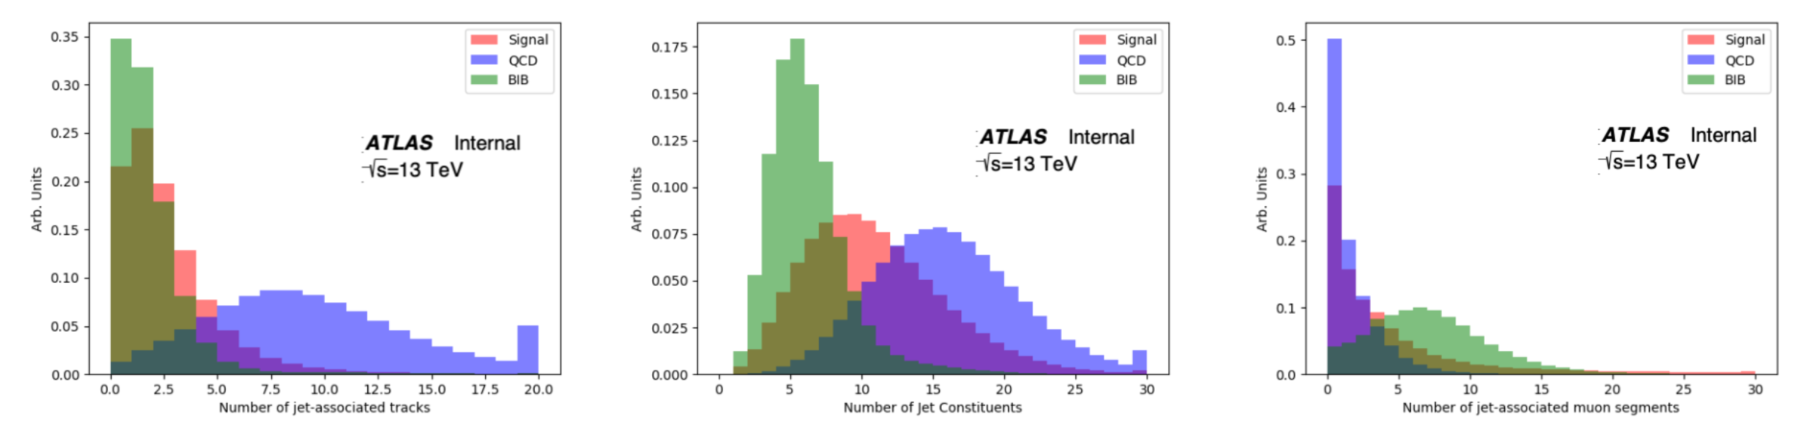
\includegraphics[width=\textwidth]{Jet-associated_number.png}
      \caption{喷注关联的径迹、拓扑集团与 μ 子段的数量}
      \label{fig:Jet-associated_number}
      \figurenote{
            左图:喷注关联的径迹数量的分布;
            中图:喷注关联的拓扑集团数量的分布;
            右图:喷注关联的 μ 子段数量的分布。
      }
\end{figure}

最后,喷注的 $p_T$、$\eta$ 与 $\phi$ 也输入神经网络进行训练。三类神经网络的喷注输入变量数量如\autoref{fig:Jet-associated_number} 所示。


\section{control region 筛选条件}
为了进行对抗训练以及计算本分析中使用的机器学习方法的系统不确定性,需要在数据和蒙特卡洛(MC)模拟中定义一个喷注控制区。
所选样本应具有统一的筛选条件,以确保喷注来源于相同的产生机制,并覆盖相同的运动学范围。
所使用的 MC 模拟样本为 JZ2W、JZ3W 和 JZ4W,它们是通用多喷注样本,包含来自质子-质子硬散射的喷注,
\pt 范围为 \SI{60}{GeV}--\SI{800}{GeV}。用于 pileup 重加权的 campaign 为 MC16a,因此控制区仅使用 2016 年的数据。

数据和 MC 样本的双喷注(dijet)筛选标准如下:
\begin{itemize}
      \item 通过 J400 HLT 触发器;
      \item 主导喷注的 $\pt > \SI{400}{GeV}$;
      \item 次主导喷注的 $\pt > \SI{60}{GeV}$;
      \item $|\eta_{\text{leading}} - \eta_{\text{subleading}}| > 3$,即两喷注在反方向上分布(back-to-back);
      \item $\frac{|\pt^{\text{leading}} - \pt^{\text{subleading}}|}{\pt^{\text{leading}} + \pt^{\text{subleading}}} < 0.3$,即主导与次主导喷注的 $\pt$ 应平衡;
      \item $m_{\text{jj}} < \SI{120}{GeV}$,即双喷注不变质量较小,符合典型的 dijet 事件特征。
\end{itemize}

此外,还应用了与预筛选类似的质量要求。通过上述筛选,选取每个事件中的前 5 个喷注作为控制区喷注。考虑到触发器要求导致主导喷注 $\pt$ 较高,因此也包含排名靠后的喷注,以获得更宽的 $\pt$ 分布。控制区中喷注的 $\pt$ 范围为 \SI{40}{GeV}–\SI{500}{GeV},以与用于训练的信号、BIB 和 QCD 样本的 $\pt$ 范围一致。

为验证该筛选方案的有效性,比较了 MC 与数据中喷注的 $\pt$ 谱。从比值图中可以看出,MC 和数据在该筛选下表现出非常相似的分布。

通过上述样本和筛选条件,最终获得约 \num{100000} 个数据喷注和 \num{200000} 个 QCD 喷注。
